\section{Bayesian Probability}
\label{sec:int_bayesian_probability}

\label{subsec:int_int_bayesian_probability}

The probability theory has its roots in the $16^{th}$ century with attempts to analyse games of chance by Cardano. It is not hard to understand why games of chance are in the foundations of the probability theory. Throughout History the concept of probability has fascinated the Human being. Luck, fate were words that reflect things we feel we have no control upon and are associated with those games, and almost paradoxically we evolved in a way that we don't feel comfortable around them. Uncertainty raises us fear and doubt, so the games of chance provide a controlled environment in which we can make our experiments with uncertainty, also by studying this games we seek to minimize the uncertainty associated with them.

\subsubsection{Kolmogorov axioms}

In spite of the fact that the problem of games of chance kept attracting numerous mathematicians (with some of the most influential ones being Fermat, Pascal and Laplace), it was not until the $20^{th}$ century that the Russian mathematician Kolmogorov laid the foundations of the modern probability theory (first published in 1933) introducing three axioms\cite{sep-probability-interpret}:

\begin{enumerate}
\item The probability of an event is a non-negative real number:
\begin{equation}
 P(A)\in\mathbb{R\;}\wedge\; P(A)\geq0
\end{equation}
This number represents the likelihood of that event happening, the greater the probability the more certain is its associated outcome. 
\item The sum of probabilities of all possible outcomes in a space is always 1 ($P(\Omega)=1$). These first two axioms leave us with the corollary that probabilities are bounded:
 \begin{equation}
0\leq P(A)\leq1
\end{equation}
\item The probability of a sequence of pairwise disjoint events is the sum these events. A corolary of this axiom is:
\begin{equation}
P(A\vee B)=P(A)+P(B) - P(A\wedge B)
\end{equation}
\end{enumerate}

The philosophical concept of probability has attracted some interpretations. Laplace was the first to provide a rigorous definition of probability (classical interpretation), that stated that the probability of an event could be obtained through the sum of elementary events divided by the sum of all possible events. Another approach to probabilities is the frequencist approach where the probability is considered an intrinsic part of a physical system that can be revealed through repeated probation. 

The Bayesian approach to the interpretation of probability is to consider the probability of an event the subjective degree of belief attributed by a Human. The subjective value attributed to an event in the Bayesian approach is called probability prior and it reflects a degree of belief in the uncertainty associated with the event before presenting any evidence. This prior probability could be obtained by counting, using a frequencist approach to determine probabilities. 

\subsubsection{Conditional Probability}
The probability after presenting some evidence is called posterior probability (or conditional probability), it is represented by $P(A|B)$ that could be read: the probability of A after evidence B is presented. This conditional probability is obtained by the product rule 
\begin{equation}
P(A|B)=\frac{P(A\wedge B)}{P(B)}
\end{equation}

\subsubsection{Bayes' Rule}
From $P(A|B)$ and $P(B|A)$ Thomas Bayes derived the Bayes' Law:

\begin{equation}
\label{eq_bayesrule}
P(A|B)=\frac{P(B|A).P(A)}{P(B)}
\end{equation}

The Bayesian probability is based in the Kolmogorov axioms, and can be seen as an extension of logic which allows to reason with propositions with an uncertain truth value ($P(true)=1$ and $P(false)= 0$) instead of being purely set based. 
The substitution of propositional variables for events is possible by a corollary of the "Stone's representation theorem for Boolean algebras".  \cite{VanRijsbergen2004} . This theorem was first proved by Stone (1936) and arose from a study of the spectral theory of operators on a Hilbert space.

If we consider $\Omega_{A}$ a finite set with n elements. A probability distribution on $\Omega_{A}$ is a function 
\begin{equation}
f:\Omega_{A}\rightarrow[0,1]
\end{equation}

%The set comprising all the distribution functions on $\Omega_{A}$ is denoted by $\mathcall{P}_{A}.
\subsubsection{Bayesian Inference}

The Bayes' Law is used to update the prior probability of an hypothesis ($h$), as evidence ($E$), is presented in a process named Bayesian Inference as in the equation \eqref{eq_bayesrule_i}.

\begin{equation}
\label{eq_bayesrule_i}
P(h|E)=\frac{P(E|h).P(h)}{P(E)}
\end{equation}

 If we have a set of hypothesis $h_{1}, h_{2}, ..., h_{n}$ to explain some evidence (symptoms of a disease, for example), we would be interested in the most probable hypothesis a posteriori (after presenting the evidence), $h_{MAP}$.

\begin{equation}
\label{eq_bayesrule_ii}
h_{MAP}= argmax_{h_{i}}\frac{P(E|h_{i}).P(h_{i})}{P(E)}
\end{equation}

As we are maximizing, we can dispose of the common denominator.

\begin{equation}
\label{eq_bayesrule_iii}
h_{MAP}= argmax_{h_{i}}P(E|h_{i}).P(h_{i})
\end{equation}

This alows for the definition of the scores 

\begin{equation}
P(E|h_{MAP}).P(h_{MAP}) 
\end{equation}

and

\begin{equation}
 P(E|\lnot h_{MAP}).P(\lnot h_{MAP})
\end{equation} 

By the law of total probability

\begin{equation}
\label{eq_law_total_probability}
1= P(h|E)+P(\lnot h|E)
\end{equation}

we can attain $P(h|E)$ and $P(\lnot h|E)$ by normalization as

\begin{equation}
\label{eq_bayesrule_alpha}
1 = \alpha < P(h|E) ; P(\lnot h|E)>
\end{equation}

This leaves us with a way to calculate $P(h|E)$ :

\begin{equation}
\label{eq_bayesrule_iiiii}
P(h|E)= \frac{P(E|h).P(h)}{P(E|h).P(h) + P(E|\lnot h).P(\lnot h)}
\end{equation}

\subsubsection{Joint Distribution}

When we need to deal with more than a one variable, the joint distribution is used to define events in terms of those variables. 
This distribution grows exponentialy (for $n$ variables, there are $2^{n}$ combinations), with the probability space of the various variables considered. If we consider the joint probability distribution between all the variables in a given domain we call this full joint probability.
%, and the tensor product is an inherent part of the definition of the joint probability space

Assuming that have three random  variables X, Y and W representing medical inferences. X represents if a person has fever, $x$ being the answer 1 (true) or 0 (false). Y represents if a person has been in a tropical region. W stands for if a person has headaches. Their joint distribution can be considered a vector with length 8 accounting for the multiple combinations of X, Y, and W. For example P(101) represents the probability of having fever and seizures without having been in a tropical region.

The joint distribution can be calculated using conditional probabilities by the chain rule. Given a set of variables $x_{1},x_{2},..., x_{n}$ :
\begin{equation}
P(\cap_{i=1}^{n}x_{i})=\prod_{i=1}^{n}P(x_{i}\vert\cap_{j=1}^{i-1}x_{j})
\end{equation}
For the last example a chain rule to calculate the joint probability would be:
\begin{equation}
\label{eq_chain_rule_example}
P(x,y,w)= P(x \vert y, w) . P(y \vert w) . P(w)  
\end{equation}

To calculate P(x) from a joint distribution we need the marginal distribution $P_{X} : x \rightarrow \sum_{w \in W} \sum_{y \in Y}P(x , y, w)$. This would require $2^{n-1}$ sums. 


\subsubsection{Conditional Independence}

When variables are independent they are uncorrelated and their marginal distributions are equal to the prior probability distribution which is attributed to each variable in cause\cite{Pearl2000}. For example: 
\begin{equation}
 P_{X}(x) = \sum_{w \in W} \sum_{y \in Y}P(x , y, w) = P(x) 
\end{equation}

So, two variables are independent iif \cite{feller1}\cite{Norvig2003}:

\begin{equation}
P(X\vert W) = P(X)
\end{equation}

That means if we are presented with three variables  X, Y and W that are conditional independent relatively to each other, their joint distribution would only account their probability prior probability functions, thus simplifying the chain rule (Equation \eqref{eq_chain_rule_example}):
\begin{equation}
P(x, y , w) = P(x) . P(y) . P(w)
\end{equation}

Although it isn't always possible to decouple variables and assume that they are conditionally independent, doing so is a way to counter the ``curse of dimensionality". 


\subsubsection{Markov Chains}
\label{subsub:MarkovChains}
Markov Chains define a system in terms of states and the probabilistic transitions from one state to another. 

\begin{figure}[h]
\centering 
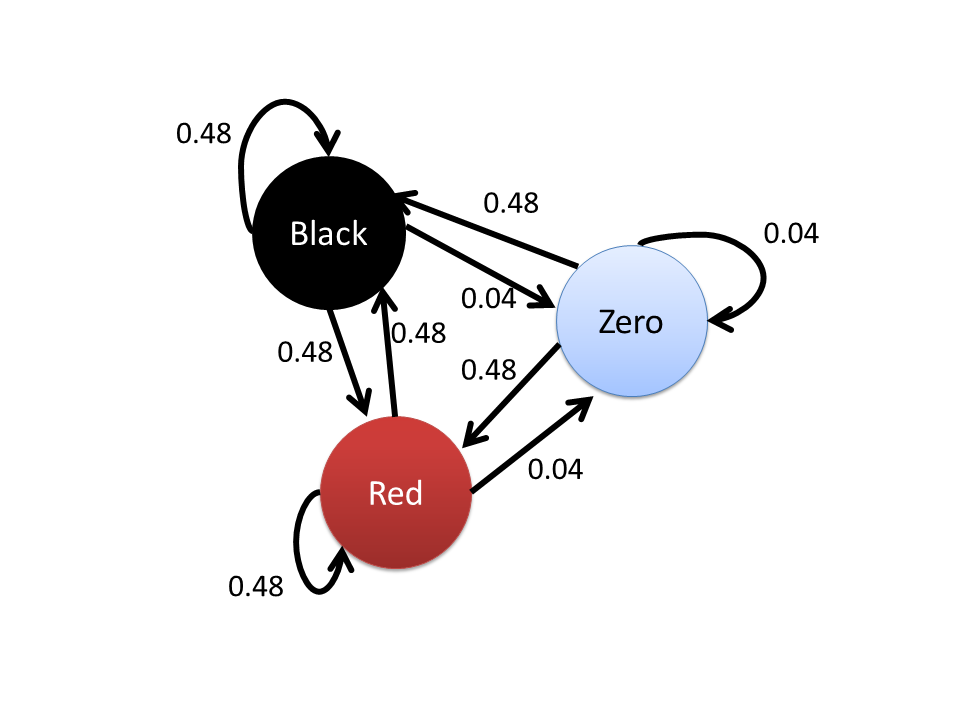
\includegraphics[scale=0.30]{Overview/Figures/RouletteMC.png}
\caption{Markov Chain of a perspective on a roulette.}
\label{fig:roulette}
\end{figure}

In 1913, at Monte Carlo Casino (Monaco), black came up twenty-six times in succession in roulette. Knowing that the probability of the ball landing on a red or on a black house is aproximately $0.48$ (the zero is a neutral house), many a gambler lost enormous sums while betting red as the they believed that the roulette was ripe with red, given the history. Players didn't want to believe that this and insisted that the roulette was biased; this became known as the Gamblers fallacy.


In the Markov Chain represented on Figure \ref{fig:roulette}, we can see that in the state black the probability of transictioning to red is the same as to stay on the state black.

Given a system represented by the states $\{ x_{0}, x_{1}, ..., x_{i}, ..., x_{n}\}$, and considering $ p_{ij}$ the probability of being in the state $j$ and transitioning to the state $i$, the mixed state vector:
\begin{equation}
\overrightarrow{x_{i}}  = \{ p_{0i}x_{0} , p_{1i}x_{1}, ... ,  p_{ii}x_{i}, ..., p_{ni}x_{n} \}
\end{equation}

represents the probabilities of the system in the that $i$ to transition to the other states. 

The law of total probability is verified as $\sum_{j=0}^{n}p_{ji}=1$, by specifying the every transition we get a stochastic matrix $P$, named the Markov matrix.

\subsubsection{Hidden Markov Models}
\ac{HMM} are a temporal statistical tool, known as Markov Model, which allows representing systems where we have a hidden layer and an output layer, that depends on the hidden layer\cite{eemcs5901}\cite{Norvig2003}. An example of a simple Markov Model could be a Markov Chain. However Markov Chains don’t have hidden layers because the state of the system is completely visible to the observer; in the roulette example (Figure \ref{fig:roulette}), we know at each moment which if we have a red house. 

In \ac{HMM}, the hidden states are not directly visible, only the output is visible\cite{citeulike:405907}. So, in order to predict the current state of the hidden layer we take into account past outputs. 



\subsection{Bayesian Networks}
\label{subsec:int_BN}

The Bayesian Networks (also referred to as Belief Networks, Probabilistic networks or causal networks) consist of an \ac{DAG} to represent a set of conditional dependencies between random variables, that provide a compact description that allows to calculate a joint probability distribution, having in mind those dependencies into account. 

The term "Bayesian Network" were first mentioned in the literature by Judea Pearl\cite{Pearl1985}. However the idea of using networks to represent conditional relationships between variables dates to the early $20^{th}$ century with Wigmore in form of charts to analyse trial evidence\cite{Kadane1996}. 

The Figure \ref{fig:inference_relationships} provides a classical example used to understand Bayesian Networks. This example is called the ``burglary network" and it is due to Judea Pearl\cite{Pearl1988}\cite{Norvig2003}. It states a case where a person is abroad and his neighbours promise to call if they hear the alarm ring. The alarm firing is correlated with the house being robbed and the possibility of an earthquake (this example is set in Los Angeles). 

\begin{figure}[h]
\centering 

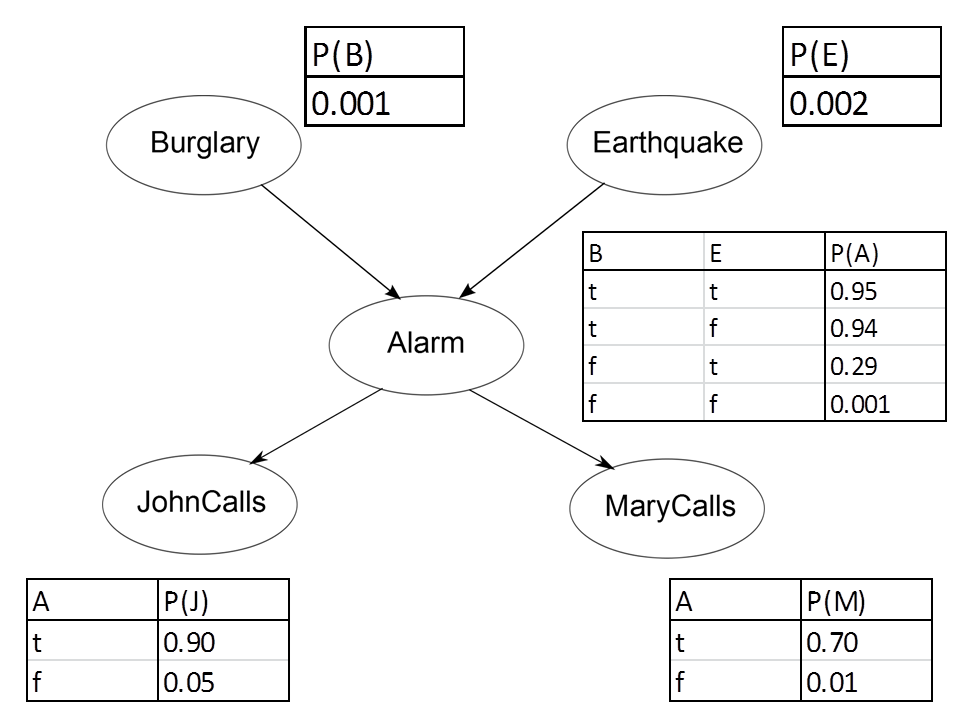
\includegraphics[scale=0.35]{Overview/Figures/BayesianNetworkExample.png}
\caption[Caption for LOF]{Burglary Network. }
\label{fig:inference_relationships}
\end{figure}
%\footnotetext{Source: \cite[Norvig and Russel 2003]{Norvig2003}}

Each node in a classical Bayesian Network represents a variable. In the example Burglary (B), Earthquake (E), Alarm (A), JohnCalls (J), and MaryCalls (M) are our random variables.
The edges represent relationships of dependency. These relationships provide elementary inference types that we can identify in the example of Figure \ref{fig:inference_relationships}. 
\begin{itemize}
\item Causation relation - A burglar(B), entering in the house makes the alarm (A), firing more likely (that's the purpose of alarms after all);
\item Diagnostic relation - The fact that the neighbours John (J) or Mary (M) call can be seen as an evidence for the alarm (A), have fired;
\item Intercausal relation - Either a burglary (B), or a earthquake (E), can cause the alarm to fire (A).
\end{itemize}

A node in a Bayesian Networks also sports a conditional probability function (represented by a \ac{CPT}). These functions consider the antecessors of the node. So for a node $X_{i}$, this would mean having access to the probability function 

\begin{equation}
\label{eq:cpt_bn}
P(X_{i} \vert Parents(X_{i} ))
\end{equation}

\ac{CPT}s for the variables considered in the previous equation. We can see that the Alarm has two antecessors (Burglary and Earthquake), so the \ac{CPT} $P(A)$, considers $P(B)$ and $P(E)$:  $P(A \vert B, E)$ as in the Equation \eqref{eq:cpt_bn}. 

The structure of the Bayesian Network allows subsets of the variables to be independent. Earthquakes don't make burglaries more likely (in the example), and Burglaries aren't known for causing earthquakes. 
Components in the networks can interact directly within a subset, despite the whole the local structure, makes this representation compact and locally structured. The set of nodes that shield a node from the rest of the network is called Markov blanket\cite{Pearl1988}. In a Bayesian Network the Markov blanket includes the parents of a node, its descendants and the parents of all its descendants. In the burglary network MaryCalls is independent of the Earthquake or the Burglary given the value of the Alarm. 

The complexity for a complete network where each variable $n$ has no more than $k$ parents is $\mathcal{O}(n.2^{k})$, this means that the complexity of a Bayesian Networks grows linearly with the number of variables, where the full joint probability on a domain grows exponentialy ($\mathcal{O}(2^{n})$). Also it is considered \cite{Pearl1985} \cite{Norvig2003} that specifying probabilities for a full joint probability table does not tally with the way human knowledge is constructed.

This makes Bayesian Networks relevant when there is a need to account for correlations between small sets of variables in a domain, providing a balance between the complexity that arises from the full joint probability table on de domain (that has the problem of exponential escalation with the increasing number of variables), and the need for models powerful enough to represent multiple dependencies. 

\subsubsection{Exact Inference}

Inference in a Bayesian Networks consists in the determination of the probability of each state in each node when there's some evidence presented.
The problem of inference in Bayesian Networks is generally NP, this made the search for optimizations and aproximations imperative. 

Considering $h$ our hypothesis variable, $e$ stands for our evidence and $Y$ are the non-evidence variables (also known as hidden or unobservable variables), we can calculate the posterior probability by enumeration, summing the terms of the full joint distribution.

\begin{equation}
P(h\vert e)=\alpha\sum_{Y}P(h,e,Y)
\end{equation}

While calculating $P(h\vert e)$ there's often repetition of calculations that cancel out. Considering an example from the burglary network, let's assume that we want to know the probability of a Burglary if both Mary and John call. This would be represented by the equation:

\begin{equation}
P(B\vert j,m)=\alpha\sum_{E}\sum_{A}P(B,j,m,A,E)
\end{equation}

By decomposing $P(B,j,m,A,E)$ using the chain rule:
\begin{equation}
P(B\vert j,m)=\alpha\sum_{E}\sum_{A}P(B).P(E).P(A\vert B,E)P(j\vert A).P(m\vert A)
\end{equation}

\begin{equation}
P(B\vert j,m)=\alpha P(B)\sum_{E}P(E)\sum_{A}P(A\vert B,E)P(j\vert A).P(m\vert A)
\end{equation}
  %imagem aqui
While computing this expression it can be seen that there are repeated sub-expressions that cancel out. In the example the following values are computed two times: 
\begin{equation}
P(j\vert A)P(m\vert A)\end{equation} and \begin{equation}P(j\vert \lnot A)P(m\vert \lnot A)\end{equation} 
Using dynamic programing can to improve the computation in the previous sittuation.

Pruning Irrelevant Variables is another way to speed up the calculation. It is considered that variables that do not belong to the evidence or the hypothesis are irrelevant unless they belong to the set comprising the ancestors of the evidence or of the hypothesis:

\begin{equation}
\label{eq:irrelevance}
Y\in\{Ancestors(\{h\}\cup e)\}
\end{equation}
In the example $P(B\vert j,m)$ $Ancestors( {B}, J, M ) = \{ A, E\}$, so there aren't irrelevant variables.
But if we take another example $P(E\vert j)$, the variable MaryCalls is irrelevant because $M \notin Antecessors( \{E\}, J ) = \{ A, B\}$.

\subsubsection{Aproximate Inference}

Given the complexity associated with exact inference, one way to fill in the \ac{CPT} of a Bayesian Network is to use approximations, namely techniques that rely on randomness. Two of this approximations techniques are:
\begin{itemize}
\item Direct Sampling Methods
\item Markov Chain Sampling
\end{itemize}

Direct sampling methods consist in using samples aquired in a training set or generated from a known probability distribution that we believe to model approximately the behaviour of the hidden variables in the network. The samples generated are used to update the \ac{CPT} of the variables in the network.

The Markov Chain Sampling assumes that the network is a system while generating samples, and it will try to make a stochastic change based on the last sample generated without disturbing evidence variables.

\subsubsection{Representing Continuous Variables}
Although the Burglary Network only has discrete stochastic variables, sometimes it's necessary to represent continuous variables.

\begin{figure}[h]
\centering 

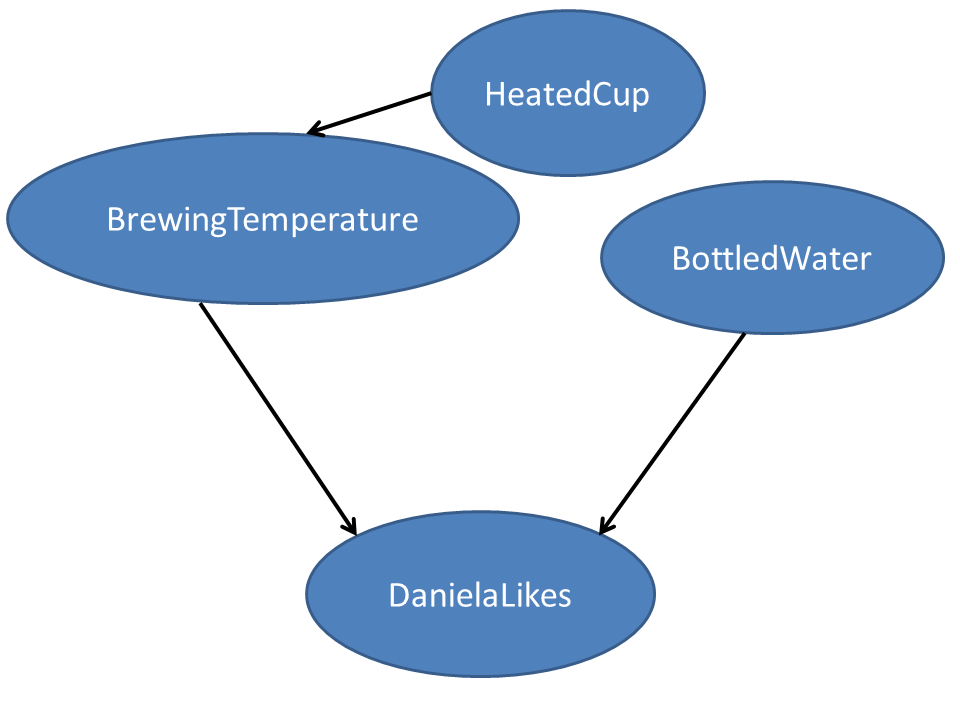
\includegraphics[scale=0.35]{Overview/Figures/TeaPreparationNetwork.png}
\caption{Tea preparation network.}
\label{fig:tea_network}
\end{figure}

One way of doing so is to create discrete intrevals, for example for the variable BrewingTemperature (representing the temperature at the end of the brewing process), in the Tea Preparation Network (Figure \ref{fig:tea_network} ), could be split in intrevals such as $T(80 > x< 85)$, but by doing so there's information that is lost.  
Other way to deal with continuous variables is to use known probabilily distributions such as the Gaussian distribution and using its parameters to model the variable. 
In the Tea preparation network where the liking of the tea is conditioned by the brewing temperature, and the brewing temperature is influenced by whether the cup was heated of not, the brewing temperature can be modeled by a Gaussian distribution. As the water is heated to a certain temperature (the mean of the distribution), the heated cup will influence directly the variations in temperature during the brewing (the more uniform the temperature during the brewing, the better), thus the standard deviation of the distribution of the Brewing temperature is conditioned by the heating of the cup.
The subject that tastes the tea will be conditioned by the use or not of bottled water and the brewing temperature. Her response to the brewing temperature can be modelled with a sigmoid function to reflect the liking or not.
A Bayesian Network with both discrete and continuous variables is called an hybrid network.


\subsubsection{Dynamic Bayesian Networks}
\ac{DBN}, also known as Two-Timeslice Bayesian Networks, are an extension of the common Bayesian Network to deal with a temporal evolution\cite{eemcs5901}. \ac{DBN} have resemblances to \ac{HMM}. More accurately we can say that \ac{HMM} are special cases of \ac{DBN}, a \ac{DBN} single discrete state variable\cite{Norvig2003}. 

The temporal dimension in \ac{DBN} is represented as time-steps. Each time step corresponds to a classical Bayesian Network, but the nodes in this Bayesian Network can have temporal links, represented as a directed edge to the next time-step, this means that these nodes will have influence on the variables of the nodes they connect with, in the following time-step.

\begin{figure}[h]
\centering 

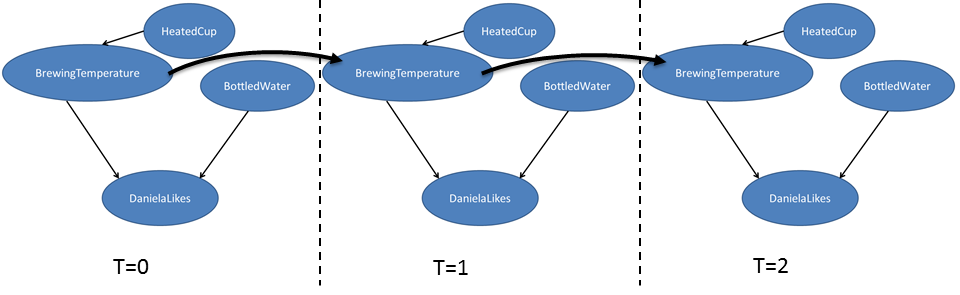
\includegraphics[scale=0.48]{Overview/Figures/TeaPreparationNetworkDBN.png}
\caption{Time evolution of the ``Tea preparation network".}
\label{fig:tea_networkdbn}
\end{figure}

In the Figure \ref{fig:tea_networkdbn} we have a possible transformation of the example of the ``Tea Preparation" to accommodate a time evolution. The variable Brewing Temperature at a given time-step will depend on the brewing temperature in the previous measurement (empiricaly we know that the temperature will not increase given the last time-step). 



\begin{comment}
Unlike the other two sampling algorithms, which generate each event from scratch, MCMC generates each event by making a random change to the preceding event. It is therefore helpful to think of the network as being in a particular current state specifying a value for every variable. The next state is generated by randomly sampling a value for one of the non-evidence variables Xi,
conditioned on the current values of the variables in the Markov
blanket of Xi. (Recall

 and requires a large amount of statistical data to 
his suggests that the elementary building blocks which make up human knowledge are not the entries of a joint-distribution table, but rather the low-order marginal and conditional probabilities defined over small clusters of propositions.


\end{comment}


%Examples???


\begin{comment}
To better enable the comparison between classical theory and quantum, Rieffel \cite[Rieffel and Polak]{Rieffel2011} considers that a "representation closer to quantum probability has advantages". This brings us to a representation of probability in a Hilbert Space and the further development of tensor product in bayesian probabilities.
\end{comment}






